\section{Auswertung}
\label{sec:Auswertung}
\subsection{Justage der Aperratur}
Zurerst werden die Parameter an dem NMR-Spektrometer so eingestellt, dass das
Signal des freien Induktionszerfall möglichst groß ist. Dafür wird als
Probe Wasser mit Kupfersulfat verwendet.
Es ergeben sich folgende Paramter:
\begin{align}
    \label{Parameter}
    f&=2169380 \, \text{Hz}\\
    p&=3°\\
    A_\text{puls}&=4.50 \, \mu \text{s}\\
    B_\text{puls}&=10.44 \, \mu \text{s}\\
    \tau&=10 \, \mu \text{s}\\
    P&=500 \, \mu \text{s}
\end{align}

\subsection{Bestimmung der longitudinalen Relaxationszeit $T_1$}
Zur Bestimmung der Relaxationszeit $T_1$ wird eine Probe mit destillierten
Wasser verwendet und die Justage der Versuchsapperatur wird für diese Probe
angepasst.
Die Messung von $T_1$ wird wie im Kapitel \ref{sec:Durchführung} beschrieben
durchgeführt, es ergeben sich folgende Messerwerte für $\tau$[ms] und $U(\tau)$[mV]

\begin{table}
  \centering
  \caption{Messwerte der Spannung in Abhängigkeit der Zeit}
  \label{tabmess1}
  \sisetup{parse-numbers=false}
  \begin{tabular}{c|c}
    \toprule
    $\tau$[ms] & $U(\tau)$[mV]\\
    \midrule
    10 & 755 \\
    20 & 745.5\\
    30 & 720\\
    40 & 705\\
    50 & 695\\
    60 & 680\\
    70 & 670\\
    80 & 662.5\\
    90 & 655.5\\
    100& 647.5\\
    150& 610\\
    200& 582.5\\
    250& 550\\
    750& 290\\
    1000& 185\\
    1250& 85\\
    1500& -250\\
    1750& -295\\
    2000& -375\\
    3000& -520\\
    4000& -730\\
    5000& -772.5\\
    \bottomrule
  \end{tabular}
\end{table}

Der erwartete Verlauf der Spannung wird durch die Formel:
\begin{align}
    \label{fidformel}
    U(\tau)=U_0 \cdot (1-2\cdot e^{\tau/T_1})
\end{align}
gegeben.

Es wird eine Funktionsanpassung durchgeführt um das $T_1$ zu bestimmen.
Der Verlauf der Messdaten mit entsprechendem Fit sind in Abbildung \ref{t1fit}
dargestellt.


\begin{figure}
\centering
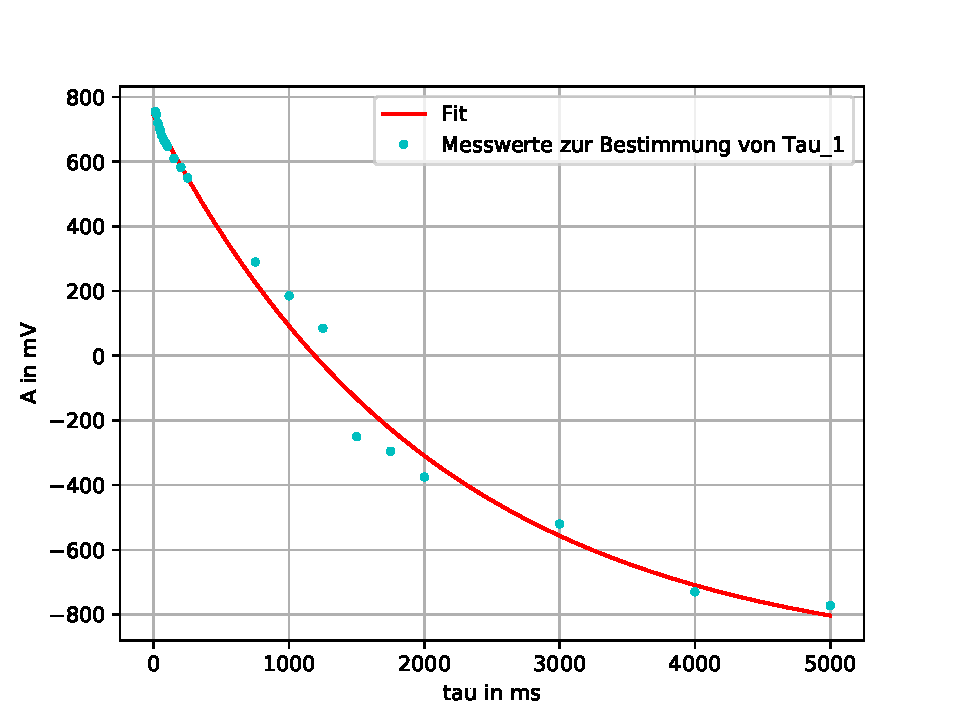
\includegraphics[width=0.8\textwidth]{/home/hubi/uni/1 Master Sem./Praktikum/MaFP_HuMa/V49/build/fit_tau_1.pdf}
\caption{Messwerte und Darstellung der Fitgergebnisse zur Berechnung
derlongitudinal Komponente $T_1$}
\label{t1fit}
\end{figure}

Dabei ergeben sich der folgende Wert für $T_1$:
$$T_1=2.1 \pm 0.2 \, \text{s}$$

\subsection{Bestimmung der transversalen Relaxationszeit $T_2$}
Die Ermittelung von $T_2$ erfolgt mittels Meiboom-Gill Methode,
welche in Kapitel \ref{sec:Theorie} erläutert wird. Es werden
die Längen der Pulse $A$ und $B$ vertauscht. Es werden
100 $B$- Pulse erzeugt und die Messwerte der Maxima für die geradezahligen
$B-$Pulse, welche in der Tabelle \ref{bpulse} angegeben sind, gespeichert.


\begin{table}
  \centering
  \caption{Messwerte der Spannung in Abhängigkeit der Zeit}
  \label{bpulse}
  \sisetup{parse-numbers=false}
  \begin{tabular}{c|c}
    \toprule
    $\tau$[ms] & $U(\tau)$[V]\\
    \midrule
    0.0005 &-0.619633 \\
    0.0405&-0.559332\\
    0.0805 &-0.547271\\
    0.1205&-0.49099\\
    0.1605&-0.49903\\
    0.2005&-0.458829\\
    0.2405&-0.47893\\
    0.2805&-0.47491\\
    0.3205&-0.458829\\
    0.3605&-0.442749\\
    0.4005&-0.446769\\
    0.4405&-0.414608\\
    0.4805&-0.430688\\
    0.5205&-0.402548\\
    0.5605&-0.398528\\
    0.6005&-0.426668\\
    0.6405&-0.370387\\
    0.6805&-0.370387\\
    0.7205&-0.358327\\
    0.7605&-0.370387\\
    0.8005&-0.358327\\
    0.8405&-0.350286\\
    0.8805&-0.350286\\
    0.9205&-0.326166\\
    0.9605&-0.318126\\
    1.0005&-0.302045\\
    1.0405&-0.330186\\
    1.0805&-0.306065\\
    1.1205&-0.294005\\
    1.1605&-0.298025\\
    1.2005&-0.285965\\
    1.2405&-0.265864\\
    1.2805&-0.269884\\
    1.3205&-0.261844\\
    1.3605&-0.261844\\
    1.4005&-0.253804\\
    1.4405&-0.225663\\
    1.4805&-0.245764\\
    1.5205&-0.225663\\
    1.5605&-0.233704\\
    1.6005&-0.226166\\
    1.6405&-0.233704\\
    1.6805&-0.221643\\
    1.7205&-0.225663\\
    1.7605&-0.201543\\
    1.8005&-0.209583\\
    1.8405&-0.181442\\
    1.8805&-0.185462\\
    1.9205&-0.193503\\
    1.9605&-0.189482\\
    \bottomrule
  \end{tabular}
\end{table}

Zur Bestimmung von $T_2$ wird eine Funktionsanpassung an die Messwerte für
den Spannungsverlauf angefertigt. Es wird ein exponentieller Abfall
für die Spannung erwartet, welcher durch die Formel:
\begin{align}
    \label{fitt2}
    U(\tau)=U_0 e^{-\tau / T_2}+U_\text{offset}
\end{align}
beschrieben wird.
Der Fit , vgl. Abbildung \ref{fittau2},  liefert folgende Werte für die Fitparameter
\begin{align*}
    U_0&=(-0.5 \pm 0.03) \, \text{V}\\
    T_2&=(1.4 \pm 0.2) \, \text{s}\\
    U_\text{offset}&=(0.06 \pm 0.03) \, \text{V}
\end{align*}



\begin{figure}
\centering
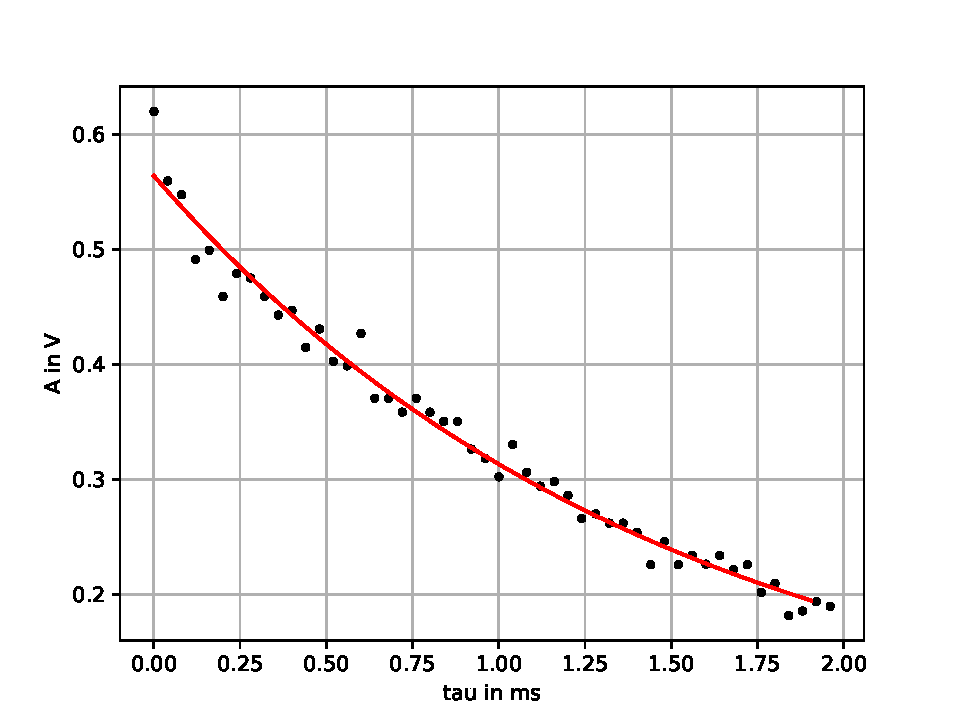
\includegraphics[width=0.8\textwidth]{/home/hubi/uni/1 Master Sem./Praktikum/MaFP_HuMa/V49/build/U_fit_Tau2.pdf}
\caption{Messwerte und Darstellung der Fitgergebnisse zur Berechnung
der transversalen Relaxationszeit $T_2$}
\label{fittau2}
\end{figure}


\subsection{Bestimmung des Feldgradienten aus der Halbwertszeit}
Der Feldgradient lässt sich mit der Breite des Echopulses
durch die Formel
$$ \frac{d \gamma G t_{1/2}}{4}=2.2$$
bestimmen. Der Probendurchmesser $d=4.4$mm und das gyromagnetische Verhältnis
$\gamma=42.58\,$MHz$\text{T}^{-1}$ sind bekannt. Die Bestimmung der
Halbwertszeit anhand des Echopulses ist in Abbildung \ref{halbw} abgebildet.

\begin{figure}[h]
\centering
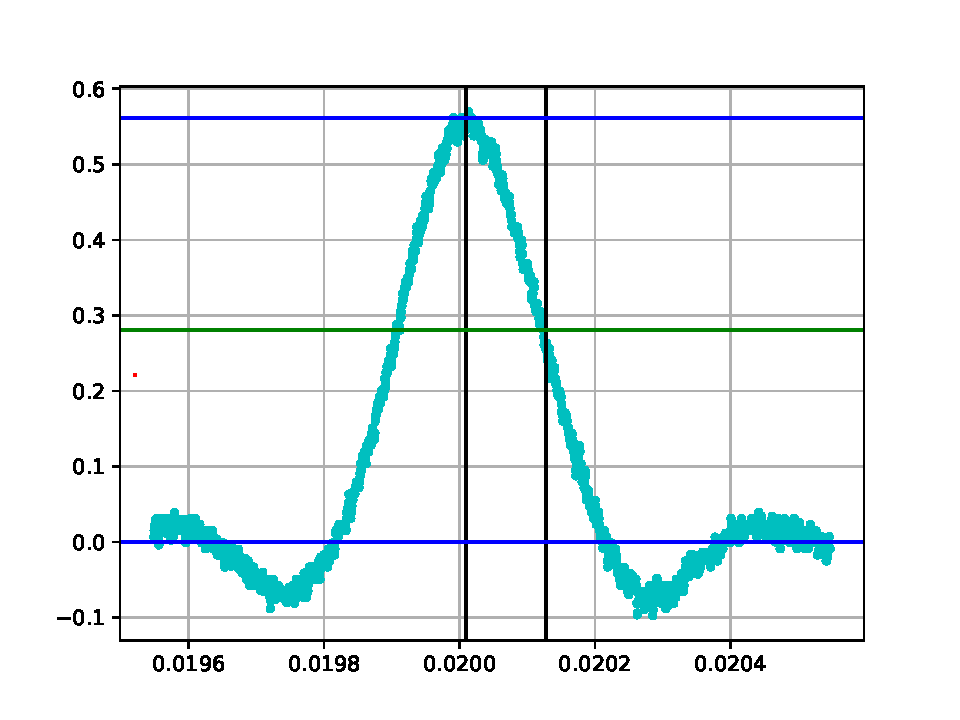
\includegraphics[width=0.8\textwidth]{/home/hubi/uni/1 Master Sem./Praktikum/MaFP_HuMa/V49/build/halbw.pdf}
\caption{Bestimmung der Halbwertszeit mit Hilfe des Spannungspulses. Der Abstand
zwischen den schwarzen Linen kennzeichnet die Spanne der Halbwertszeit}
\label{halbw}
\end{figure}
Die Halbwertszeit beträgt $t_{1/2}= 11.7\cdot 10^{-5}\,$s, sodass nun für den
Feldgradienten folgt:
$$G=-0.41\, \text{T}\text{m}^{-1}$$

\subsection{Ermittlung der Diffusionskonstante mit dem Spin-Echo Verfahren}
Die Bestimmung der Diffusionskonstante erfolgt mit dem Spin-Echo Verfahren,
die dafür aufgenommenen Messwerte finden sich in der Tabelle \ref{Tabdiff},
bzw. die graphische Darstellung in Abbildung \ref{fitd}. Auf
die Messwerte wird ein Fit der Funktion
$$U(\tau)=U_0 e^{-\tau / T_2}e^{-c\tau^3}+U_\text{offset}$$
angewendet. Es ergeben sich für die Fitparameter:
\begin{align*}
U_0&=(0.7 \pm 0.2 )\, \text{V},\\
c&= (33 \pm 0.033)\,\cdot 10^{5}/\text{s}^3.
\end{align*}
Die Diffusionskonstante kann aus dem Fitparameter $c$ berechnet werden:
$$c=\frac{D \gamma^2 G^2}{12} \rightarrow D=\frac{12c}{\gamma^2 G^2}= (1.37 \pm 0.09)\cdot 10^{-9}/\text{s}$$



\begin{table}
  \centering
  \caption{Messwerte der Spannung in Abhängigkeit der Zeit}
  \label{tabmess1}
  \sisetup{parse-numbers=false}
  \begin{tabular}{c|c}
    \toprule
    $\tau$[ms] & $U(\tau)$[mV]\\
    \midrule
5&   700\\
7.5& 685\\
9  & 660\\
10 & 630\\
12 & 590\\
14 & 540\\
16 & 410\\
18 & 350\\
20 & 278\\
22 & 213\\
23 & 175\\
24 & 138.5\\
25 & 130.6\\
26 & 98.125\\
27 & 81.25\\
28 & 72.5\\
29 & 58.75\\
30 & 51.875\\
31 & 45     \\

\bottomrule
\end{tabular}
\end{table}

\begin{figure}[h]
\centering
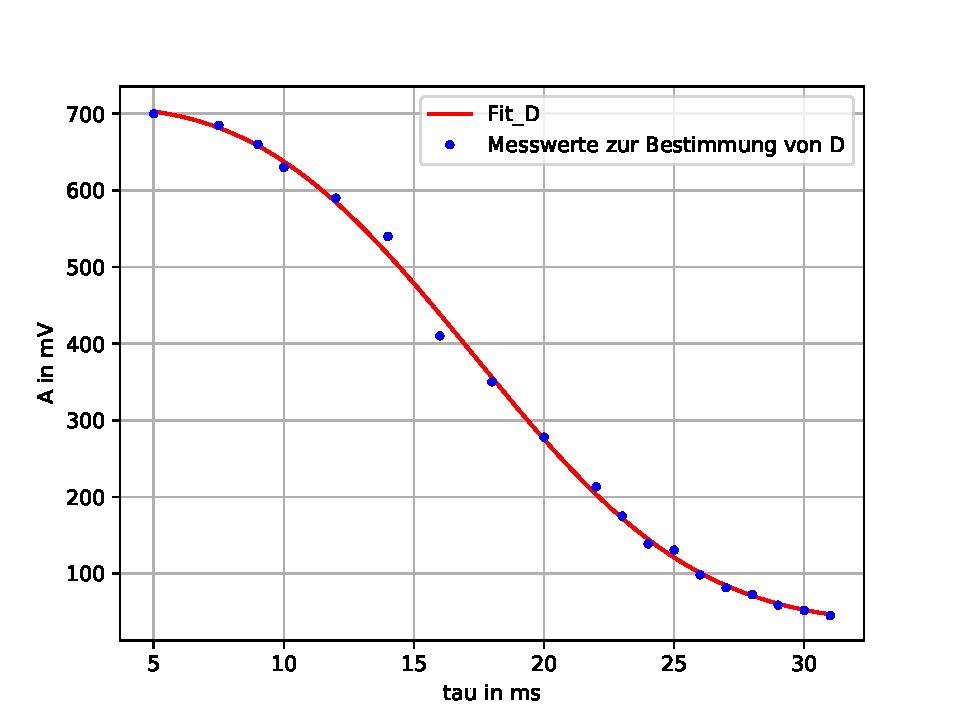
\includegraphics[width=0.8\textwidth]{/home/hubi/uni/1 Master Sem./Praktikum/MaFP_HuMa/V49/build/plot_diff.pdf}
\caption{Fit zur Bestimmung der Diffusionskonstante}
\label{fitd}
\end{figure}

\subsection{Bestimmung der Viskosität und des Molekülradius von Wasser}
Zur Messung der Viskosität wird ein Ubbelohde Viskosimeter verwendet,
wodurch durch eine einfache Zeitmessung die Viskosität bestimmt werden kann.
Die gemessene Zeit die das Wasser braucht um durch die
Kapillare zu fließen beträgt $t=931\,$s, welches sich mit der Formel für
dieses Viskosimeter in eine Viskosotät umrechnen lässt:
$$ \eta=\alpha \rho (t- \delta).$$
Die Dichte der Flüssigkeit beträgt hier mit $\rho=0.997\approx 1$g$/$c$\text{m}^3$,
sodass für die die Eichkonstante der Apperatur den wesentlichen Anteil
der Viskosität ausmacht. Das $\delta$ ist eine Korrekturglied und beträgt hier
$\delta=0.5\, \text{s}$, für die Viskosität folgt, unter der Annahme das die Zeit auf
1s genau bestimmt werden konnte:
$$\eta=(0.949 \pm1)\,\text{mPa}\,\text{s} $$

Mit Hilfe der Viskosität lässt sich der Molekülradius $r$ von  Wasser berechnen:
$$r=\frac{kT}{6 \pi D \eta}=(1.7\pm 0.6)\cdot 10^{-11}\, \text{m}$$
Hierfür wird eine Temperatur von $T=25°C$ angenommen.
